\documentclass[tikz,border=8pt]{standalone}
\usepackage{amsmath}
\usetikzlibrary{arrows.meta,calc,fit,backgrounds}

\definecolor{forwardblue}{RGB}{50,92,140}
\definecolor{backorange}{RGB}{204,93,39}
\definecolor{autoteal}{RGB}{55,132,125}
\definecolor{lossviolet}{RGB}{126,80,126}
\definecolor{boxfill}{RGB}{247,250,252}
\definecolor{modelfill}{RGB}{232,245,243}
\definecolor{autofill}{RGB}{232,247,245}
\definecolor{lossfill}{RGB}{238,219,238}
\definecolor{notefill}{RGB}{255,249,230}

\begin{document}
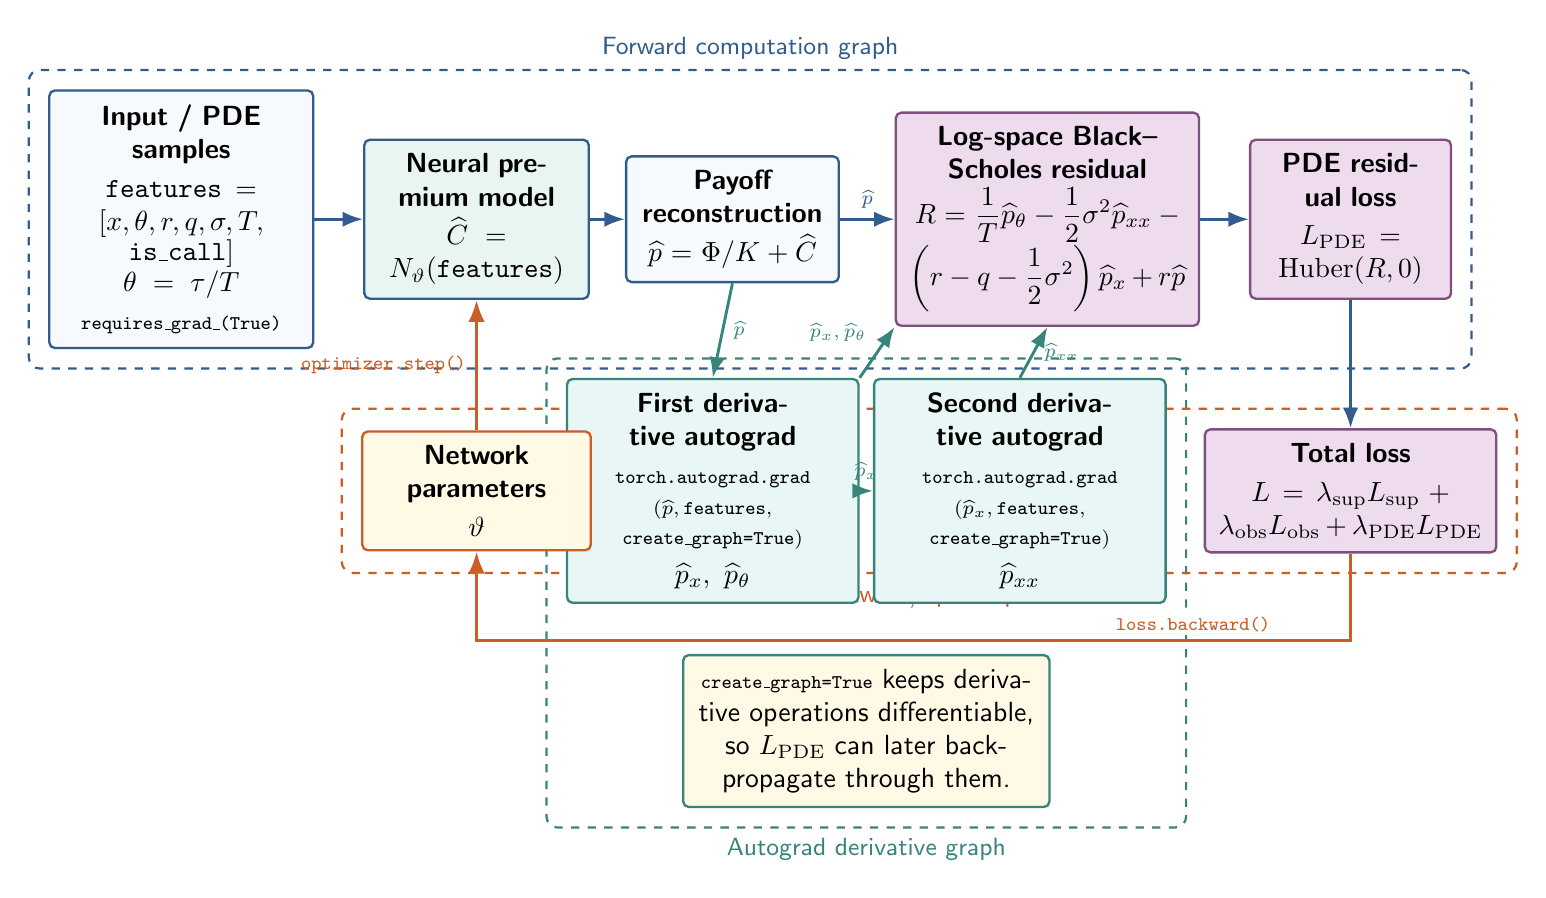
\begin{tikzpicture}[
    font=\sffamily,
    box/.style={
        draw=#1,
        fill=boxfill,
        rounded corners=2pt,
        line width=0.85pt,
        align=center,
        inner sep=5pt
    },
    box/.default=forwardblue,
    fwd/.style={-{Latex[length=2.6mm]}, forwardblue, line width=1.05pt},
    grad/.style={-{Latex[length=2.6mm]}, autoteal, line width=1.05pt},
    back/.style={-{Latex[length=2.8mm]}, backorange, line width=1.15pt},
    lane/.style={draw=#1, rounded corners=4pt, dashed, line width=0.8pt, inner sep=7pt},
    lane/.default=forwardblue
]

% Forward lane.
\node[box=forwardblue, text width=3.0cm] (features) at (-7.0,2.4)
    {\textbf{Input / PDE samples}\\[2pt]
    $\texttt{features}=[x,\theta,r,q,\sigma,T,$\\[-1pt]
    $\texttt{is\_call}]$\\[-1pt]
    $\theta=\tau/T$\\[2pt]
    {\scriptsize\texttt{requires\_grad\_(True)}}};

\node[box=forwardblue, fill=modelfill, text width=2.5cm] (model) at (-3.25,2.4)
    {\textbf{Neural premium model}\\[2pt]
    $\widehat C=N_{\vartheta}(\texttt{features})$};

\node[box=forwardblue, text width=2.35cm] (recon) at (0.0,2.4)
    {\textbf{Payoff reconstruction}\\[2pt]
    $\widehat p=\Phi/K+\widehat C$};

\node[box=lossviolet, fill=lossfill, text width=3.5cm] (residual) at (4.0,2.4)
    {\textbf{Log-space Black--Scholes residual}\\[2pt]
    $\displaystyle
    R=\frac{1}{T}\widehat p_{\theta}
    -\frac{1}{2}\sigma^2\widehat p_{xx}
    -\left(r-q-\frac{1}{2}\sigma^2\right)\widehat p_x
    +r\widehat p$};

\node[box=lossviolet, fill=lossfill, text width=2.2cm] (pdeloss) at (7.85,2.4)
    {\textbf{PDE residual loss}\\[2pt]
    $L_{\mathrm{PDE}}=\operatorname{Huber}(R,0)$};

% Autograd lane.
\node[box=autoteal, fill=autofill, text width=3.35cm] (gradone) at (-0.25,-1.05)
    {\textbf{First derivative autograd}\\[2pt]
    {\scriptsize\texttt{torch.autograd.grad}}\\[-1pt]
    {\scriptsize$(\widehat p,\texttt{features},$}\\[-1pt]
    {\scriptsize$\texttt{create\_graph=True})$}\\[2pt]
    $\widehat p_x,\ \widehat p_{\theta}$};

\node[box=autoteal, fill=autofill, text width=3.35cm] (gradtwo) at (3.65,-1.05)
    {\textbf{Second derivative autograd}\\[2pt]
    {\scriptsize\texttt{torch.autograd.grad}}\\[-1pt]
    {\scriptsize$(\widehat p_x,\texttt{features},$}\\[-1pt]
    {\scriptsize$\texttt{create\_graph=True})$}\\[2pt]
    $\widehat p_{xx}$};

\node[box=autoteal, fill=notefill, text width=4.3cm] (note) at (1.7,-4.1)
    {{\scriptsize\texttt{create\_graph=True}} keeps derivative operations differentiable, so $L_{\mathrm{PDE}}$ can later backpropagate through them.};

% Training/update lane.
\node[box=lossviolet, fill=lossfill, text width=3.35cm] (totalloss) at (7.85,-1.05)
    {\textbf{Total loss}\\[2pt]
    $L=\lambda_{\mathrm{sup}}L_{\mathrm{sup}}
    +\lambda_{\mathrm{obs}}L_{\mathrm{obs}}
    +\lambda_{\mathrm{PDE}}L_{\mathrm{PDE}}$};

\node[box=backorange, fill=notefill, text width=2.55cm] (params) at (-3.25,-1.05)
    {\textbf{Network parameters}\\[2pt]
    $\vartheta$};

% Forward computation arrows.
\draw[fwd] (features) -- (model);
\draw[fwd] (model) -- (recon);
\draw[fwd] (recon) -- node[above, font=\scriptsize] {$\widehat p$} (residual);
\draw[fwd] (residual) -- (pdeloss);
\draw[fwd] (pdeloss) -- (totalloss);

% Autograd derivative arrows.
\draw[grad] (recon.south) -- node[right, font=\scriptsize] {$\widehat p$} (gradone.north);
\draw[grad] (gradone) -- node[above, font=\scriptsize] {$\widehat p_x$} (gradtwo);
\draw[grad] (gradone.north east) -- node[above left, font=\scriptsize] {$\widehat p_x,\widehat p_{\theta}$} (residual.south west);
\draw[grad] (gradtwo.north) -- node[right, font=\scriptsize] {$\widehat p_{xx}$} (residual.south);

% Backward/update path.
\draw[back] (totalloss.south) -- ++(0,-1.10) -| (params.south);
\node[font=\scriptsize, text=backorange, fill=white, inner sep=1pt] at (5.85,-2.75)
    {\texttt{loss.backward()}};
\draw[back] (params.north) -- node[left, font=\scriptsize]
    {\texttt{optimizer.step()}} (model.south);

\begin{scope}[on background layer]
    \node[lane=forwardblue, fit=(features)(model)(recon)(residual)(pdeloss),
        label={[font=\sffamily\small, text=forwardblue]above:Forward computation graph}] {};
    \node[lane=autoteal, fit=(gradone)(gradtwo)(note),
        label={[font=\sffamily\small, text=autoteal]below:Autograd derivative graph}] {};
    \node[lane=backorange, fit=(params)(totalloss),
        label={[font=\sffamily\small, text=backorange]below:Backward/update path}] {};
\end{scope}

\end{tikzpicture}
\end{document}
